%!TEX root = ../template.tex
%%%%%%%%%%%%%%%%%%%%%%%%%%%%%%%%%%%%%%%%%%%%%%%%%%%%%%%%%%%%%%%%%%%%
%% chapter4.tex
%% NOVA thesis document file
%%
%% Chapter with lots of dummy text
%%%%%%%%%%%%%%%%%%%%%%%%%%%%%%%%%%%%%%%%%%%%%%%%%%%%%%%%%%%%%%%%%%%%
\chapter{Background}
\label{cha:background}
After the presentation of the problem and the motivations behind it, in this chapter will be introduced key concepts of Human-Computer Interaction, as well as, a briefly contextualization of the OutSystems Platform Background that are indispensable for the comprehension and progression of this study.

\section{Human-Computer Interaction}
\label{sec:human_computer_interaction}
Since the goal of this project is to improve and extend the visual language that gives to the user the possibility to construct queries through manipulation of visual components of graphical user interface. Human-computer interaction concepts, rules and techniques are fundamental to design and evaluate any possible solution to this problem. Thus, following, will be presented a summary of human-computer interaction topics taken into account throughout the design and development of this project.

Although computer systems have been designed by humans, these two parts of human-computer interaction do not communicate through the same language. Nonetheless, these type of systems were created to support, in a transparent way, human’s tasks and requirements, forgiving careless mistakes. \cite{humanComputerInteraction} Thus, human-computer interaction fields aim to study the relationship of users and computer systems, in the context of the users’ desired tasks, in order to “unfold and reveal challenges and insights, and to instrument appropriate solutions for alleviating the current obstacles to the access and use of advanced information technologies” \cite{userInterfacesForAll_newPerspectivesIntoHumanComputerInteraction}. 

%\textit{Dix et al.} \cite{humanComputerInteraction} reinforce this too, saying that “HCI involves the design, implementation and evaluation of interactive systems in the context of the user’s task and work”.

\subsection{Interaction Models}
\label{subsec:interaction_models}

Therefore, have been proposed interaction models to represent the intention of a user to perform a certain task on a system. One of the most influential is Norman’s model, that characterize the interaction of a user with a system beyond execution-evaluation cycles. \cite{humanComputerInteraction} Thereby, the execution is a flow when the user interacts with the system, and the evaluation phase comprise the presentation and the interpretation of the system output. However, this model only represents the interaction from the users’ point of view. Thereupon, Abowd and Beale \cite{userSystemsAndInterfaces_aUnifyingFrameworkForInteraction} proposed an extension of this model where it is possible to view how the system communicates through the interface.

In this approach, represented in \ref{fig:abowdAndBealeModel}, after the user has defined his goal and respective tasks to achieve it, he transmits his intention (articulation) through input language, and after this, that information is translated to system language (performance), ending the execution phase. Secondly, the result of the action executed by the system is presented (presentation) and the user observes it (observation), ending the evaluation phase.

\begin{figure}[htbp]
	\centering
	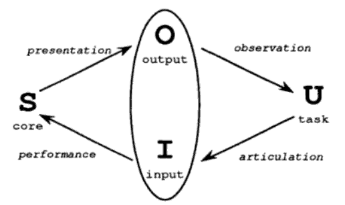
\includegraphics[height=1.75in]{abowdAndBealeModel}
	\caption{Interaction Model proposed by Abowd and Beale \cite{userInterfacesForAll_newPerspectivesIntoHumanComputerInteraction} (Based on Norman’s Model)}
	\label{fig:abowdAndBealeModel}
\end{figure}

These models are useful to understand two concepts that cannot be forgotten when a system is being designed, since these are two effects that designers want to reduce as much as possible, in order to optimize the effectiveness of the human-computer dialogue. Following, these concepts will be described respecting \textit{Dix et al.} \cite{humanComputerInteraction} definition:

\begin{itemize}
    \item \textbf{Gulf of execution}: “Difference between the user’s formulation of the actions to reach the goal and the actions allowed by the system. If the actions allowed by the system correspond to those intended by the user, the interaction will be effective.”
    \item \textbf{Gulfs of evaluation}: “Distance between the physical representation of the system state and the expectation of the user. If the user can readily evaluate the presentation in terms of his goal, the gulf of evaluation is small.”
\end{itemize}

\subsection{Main Concepts}
\label{subsec:main_concepts}
The \textbf{Usability} of a system is one of the most important concepts in human-computer interaction, that can not be forgotten on the design process, since its attributes must be taken into account performing also a guidance function through all this process. This concept was standardized in ISO-9241 \cite{iso9241-11_2018} as “extent to which a system, product or service can be used by specified users to achieve specified goals with effectiveness, efficiency and satisfaction in a specified context of use”.

However, as referred by Nielsen \cite{usabilityEngineering}, usability is not a single-dimensional property, being always associated with its attributes, that characterize the user accessibility when is using the system into five different points: